\chapter{Fundamentação Teórica}
\phantom{0}

Neste capítulo são detalhados os tópicos necessários para compreensão das técnicas utilizadas na elaboração do método proposto. As seções seguintes abordam conceitos sobre a Síndrome do Olho Seco e o exame oftalmológico, métodos de análise de textura baseado em diversidade filogenética e em estatística espacial, seleção de características, técnicas de reconhecimento de padrões, e as métricas de desempenho para validação dos resultados.

\section{Filme Lacrimal, Imagem e Síndrome do Olho Seco}

A relação da estrutura do filme lacrimal e as imagens adquiridas, é de suma importância para o entendimento da grande variedade e diferenças sutis que podem representar as categorias presente na camada lipídica do filme lacrimal.

\subsection{Filme Lacrimal}
\label{sec:filmeLacrimal}

O filme lacrimal é responsável por umidificar a superfície ocular sendo composto por lágrimas, secretadas pela glândula lacrimal, distribuídas através do movimento de piscar dos olhos \cite{remeseiro2014methodology}. As principais funções do filme lacrimal são: óptico, metabólico (fornece nutrição corneal), antimicrobiano (devido à presença de enzimas e imunoglobulina A) e como barreira mecânica (elimina detritos celulares e substâncias ambientais) \cite{dry2007definition}. A sua estrutura é composta por três camadas \cite{rolando2001ocular}, ilustrada na Figura~\ref{fig:EstruturaFilmeLacrimal}:

\begin{itemize}
    \item Camada mucosa: é a camada mais interna em contato com a superfície ocular, responsável pela adesão das lágrimas aos olhos, formando uma película protetora transparente que umidifica o epitélio da córnea;
    \item Camada aquosa: é a camada intermediária, produzida pelas glândulas lacrimais e contém alto teor aquoso, além de ser responsável por assegurar a nutrição da córnea e proteger o olho de corpos estranhos;
    \item Camada lipídica: é a camada mais externa e está em contato com o ambiente. Ela apresenta como função a prevenção da evaporação da água ocular, diminuição da tensão superficial que ajuda na estabilidade vertical e a lubrificação dos cílios quando passam pela superfície ocular.
\end{itemize}

\begin{figure}[!ht]
    \centering
    \caption[Estrutura do filme lacrimal.]{Estrutura do filme lacrimal.}
    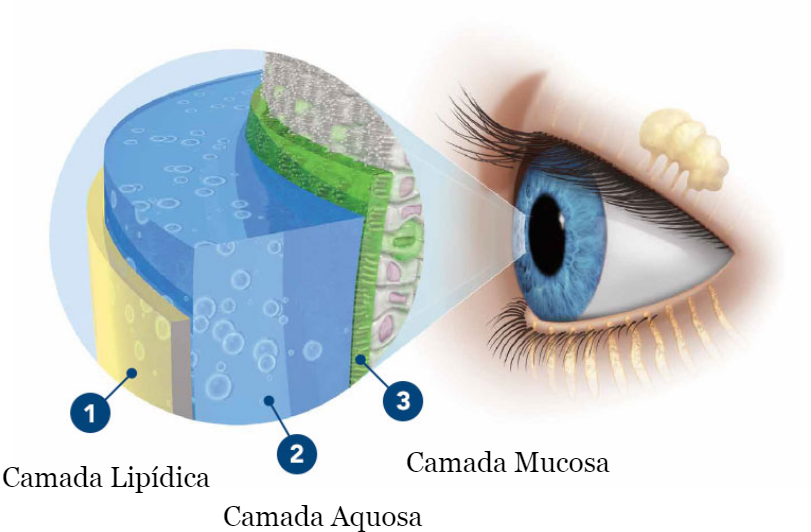
\includegraphics[width=0.6\textwidth]{figs/ImagemCamadas.png}
    \legend{Fonte: Adaptado de \cite{UnderstandingDryEye}.}
    \label{fig:EstruturaFilmeLacrimal}
\end{figure}

A Síndrome do Olho Seco evaporativo é causada pela deficiência da camada lipídica. Assim, a avaliação dessa camada é uma das formas utilizadas para avaliar o filme lacrimal \cite{korb2002tear}.

\subsection{Imagens e Síndrome do Olho Seco}
\label{sec:imgPatologia}

A Síndrome do Olho Seco é uma doença multifatorial da superfície ocular que resulta em desconforto, distúrbios visuais e instabilidade do filme lacrimal. Embora haja portadores assintomáticos, a maioria tem como principais sintomas: sensação de corpo estranho, queimação, instabilidade do filme lacrimal com potencial dano à superfície ocular, prurido, fotofobia, embaçamento visual e lacrimejamento excessivo, o que pode causar impacto na qualidade de vida. Este distúrbio é mais comum em adultos com mais de 40 anos e afeta principalmente as mulheres \cite{valim2015current}.

Existem duas categorias da Síndrome do Olho Seco, de acordo com a classificação do DEWS (\textit{International Workshop on Dry Eye} - Workshop Internacional sobre Olho Seco): deficiência aquosa e aumento da evaporação. A principal causa da Síndrome do Olho Seco do tipo de deficiência aquosa é a síndrome de Sjögren (SS). Além da SS, outras doenças causam a diminuição da produção das lágrimas como: lúpus eritematoso sistêmico, reumatoide, esclerose sistêmica, sarcoidose, artrite, linfoma, diabetes, episclerite, HIV ou infecções por vírus da hepatite C, deficiência da glândula lacrimal, obstrução do ducto lacrimal, hipossecreção reflexa e uso de medicações sistêmicas \cite{dry2007definition, lemp2012distribution, sivaraj2007ocular, waszczykowska2013prevalence, fox1994systemic}.

A Síndrome do Olho Seco evaporativo pode ser causado por várias outras doenças, como blefarite, psoríase, rosácea, dermatite seborreica, conjuntivite alérgica e distúrbios palpebrais (paralisia do nervo facial, doença de Graves), uso prolongado de lentes de contato e medicamentos de uso tópico e uso sistêmico. Entretanto, estudos mostram que ambos os tipos geralmente coexistem, e a forma isolada evaporativa é mais comum que a deficiência isolada aquosa \cite{dry2007definition, lemp2012distribution, fonseca2010olho}.

O diagnóstico da patologia é uma tarefa difícil devido à sua etiologia multifatorial e vários testes clínicos, que podem ser utilizados tanto para o diagnóstico quanto para o tratamento. A avaliação dos padrões de interferência que categorizam a camada lipídica através da classificação do filme lacrimal é um dos testes mais comuns para diagnosticar a Síndrome do Olho Seco \cite{GUILLON1998S31}. Essa avaliação pode ser realizada utilizando diferentes tipos de instrumentos: Tearscope Plus, Interferômetro Doane, Tomografia de Coerência Óptica (OCT), etc.

%A espessura e a regularidade da camada lipídica são categorizadas observando a aparência e a cor do padrão de interferência entre a camada lipídica e as camadas subjacentes.O instrumento usado em conjunto com um biomicroscópio não iluminado fornece ampliação adequada da imagem.

O Interferômetro Doane apresentado e desenvolvido por Doane \cite{doane1989instrument}, consiste originalmente em uma fonte de luz e um sistema de observação que captura a aparência do filme lacrimal usando um sistema baseado em vídeo. Este modelo permite que as mudanças dinâmicas que ocorrem ao longo do tempo sejam gravadas, permitindo que clínicos avaliem rapidamente a espessura da camada lipídica.

\citeonline{thai2004effect} utilizaram o Interferômetro para medir a taxa de evaporação, características de desgaste e mudanças na camada lipídica do filme lacrimal. Para isto, eles propuseram um sistema para classificação do filme lacrimal em imagens de diferentes categorias. Com base em tal estudo, uma nova escala de classificação composta por cinco categorias foi proposta em \cite{remeseiro2015automatic} uma vez que o uso de uma câmera digital produziu mudanças nos detalhes vistos nas imagens digitais. Essas categorias são: detritos, franjas finas, coalescente de franjas finas, franjas fortes e coalescente de franjas fortes.

O Tearscope Plus é o instrumento projetado por Guillon para avaliação rápida da espessura da camada lipídica \cite{GUILLON1998S31}. Ele projeta uma fonte cilíndrica de luz fluorescente branca fria sobre a camada lipídica e, portanto, qualquer fenômeno observado é exclusivo de sua fonte de luz específica. Em geral, as imagens do Tearscope são analisadas durante a realização do exame, sem qualquer processo de aquisição. No entanto, existem alguns estudos que utilizaram procedimentos de aquisição de vídeo/imagens \cite{efron2012}, \cite{king1999three}, que auxiliam o observador a classificar corretamente os padrões e são indispensáveis para a análise computacional.

Os conjuntos de imagens capturadas pelo Tearscope Plus podem conter cinco categorias: malhas abertas, malhas fechadas, ondas, amorfa e de franja. Em ambos instrumentos, a variabilidade da aparência dos padrões de interferência da camada lipídica resultam em grandes variações inter e intra observadoras. Portanto, a classificação visual dos padrões é uma tarefa clínica difícil, especialmente com camadas lipídicas mais finas que não possuem características de cor e/ou morfológicas \cite{garcia2013new}.

Nas próximas seções desse capítulo são apresentados os conceitos teóricos utilizados pelo método proposto para a classificação automatizada da camada lipídica em imagens do filme lacrimal. Os aspectos fisiológicos dos olhos expostos nessa seção serão levados em consideração para o aperfeiçoamento das técnicas propostas no método apresentado no próximo capítulo.

\section{Processamento Digital de Imagens}
\label{sec:PDI}

Em geral, o processamento digital de imagens é definido como um conjunto de técnicas computacionais que transformam uma imagem de entrada em uma saída desejada \cite{gonzalez2010processamento}. Esse conjunto de técnicas possibilita extrair e identificar informações das imagens e melhorar a qualidade visual de aspectos estruturais, facilitando a percepção humana e a interpretação automática por meio de máquinas \cite{pedrini2008analise}.

O principal objetivo do processamento de imagens é auxiliar a compreensão do mesmo, entretanto, existem vários algoritmos com finalidades muito específicas, que juntos formam a metodologia final. Portanto, uma metodologia difere de outra na maneira que compõe seus passos ou ferramentas, mas tipicamente obedecem as etapas apresentadas por Gonzalez e Woods (2010)\nocite{gonzalez2010processamento}, conforme apresentado na~\autoref{fig:passosProcessamentoImagens}.

As etapas fundamentais para resolução do problema, são\cite{gonzalez2010processamento}: aquisição das imagens digitais, pré-processamento, segmentação, representação, descrição e, reconhecimento e interpretação. O resultado gerado por uma etapa é utilizado como entrada na etapa seguinte onde cada entrada e resultado pode ou não ser uma imagem digital. Uma metodologia de processamento de imagens pode conter apenas um subconjunto de todas as etapas apresentadas \cite{BRAZ:2014}.

\begin{figure}[ht!]    
	\centering
	\caption{Etapas fundamentais em processamento digital de imagens.}
	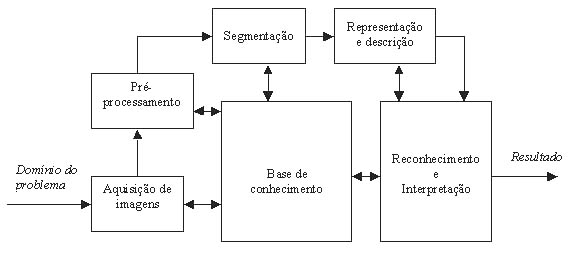
\includegraphics[width=0.90\textwidth]{figs/passosProcessamentoImagens.png}
	\legend{Fonte: Adaptado de \cite{gonzalez2010processamento}.}
	\label{fig:passosProcessamentoImagens}
\end{figure}

As etapas necessárias após a definição e delimitação do problema, foram: segmentação, extração de características, seleção de características e reconhecimento de padrões, com base no modelo apresentado. Portanto, no restante deste capítulo são abordados os aspectos teóricos das técnicas utilizadas no método proposto desta dissertação.

\begin{comment}
\section{Pré-processamento}
\label{sec:preprocessamento}

Nesta seção são apresentadas as técnicas de melhoramento de imagens utilizadas no método proposto, visando aprimorar o desempenho da segmentação, extração de características e reconhecimento de padrões. Para o desenvolvimento do método foram utilizadas técnicas de realce para o tratamento do contraste das imagens e quantização para a digitalização dos valores de amplitude.  

%que utiliza o valor máximo e mínimo da imagem digitalizada e divide a escala de cinza em intervalos iguais de acordo com o número de \textit{bits} definidos. Uma forma de calcular 

\subsection{Filtro Homomórfico}

O filtro homomórfico é usualmente utilizado em melhoramento de imagens digitais. Essa técnica analisa separadamente as informações de reflectância e iluminação, obtendo uma imagem com realce das altas frequência (reflectância) e atenuação das baixas frequências (iluminação). A iluminância $i(x,y)$ representa a quantidade de luz que incide sobre o \textit{pixel}. Já a reflectância $r(x,y)$ indica quanto dessa luz incidente é refletida. A ideia central é que a iluminação varie pouco ao longo da imagem em relação à reflectância.

De acordo com Melo et al. (2005)\nocite{de2005system}, a o filtro homomórfico tem como entrada a função $f(x,y)$, que representa a imagem de entrada em níveis de cinza. Em seguida, os valores dos \textit{pixels} são convertidos para o logaritmo natural (\autoref{eq:logaritmo}), onde ocorre a separação dos componentes de iluminação e reflectância. Na imagem logarítmica é aplicado o filtro passa-baixa\footnote{permite a passagem dos componentes de mais baixa frequência, atenuando o contraste.} e o filtro passa-alta\footnote{permite a passagem dos componentes de alta frequência com facilidade, porém reduz a amplitude das frequências abaixo da frequência de corte.} resultando em $log(i(x,y))$ e $log(r(x,y))$, respectivamente.

\begin{equation}
\label{eq:logaritmo}
f(x, y) = log(1 + f(x, y))
\end{equation}

As imagens resultantes dos filtros passa-baixa e passa-alta são multiplicadas por valores $\alpha$ e $\beta$, onde $\alpha$ < 1 e $\beta$ > 1, respectivamente. Dessa forma, diminuirá os limites amplos de intensidade em $log(i(x,y))$ e aumentará o contraste local em $log(r(x,y))$. Posteriormente, $\alpha \times log(i(x,y))$ e $\beta \times log(r(x,y))$ são somadas e normalizadas entre faixa de valores 0 e 1. Finalmente, é calculado o exponencial da imagem normalizada (evita tender ao infinito), seguida da normalização para os níveis de cinza (0 - 255) e aplicação da equalização do histograma. Na~\autoref{fig:filtroH2} é apresentado o esquema de aplicação do filtro homomórfico.

\begin{figure}[ht!]
    \centering
    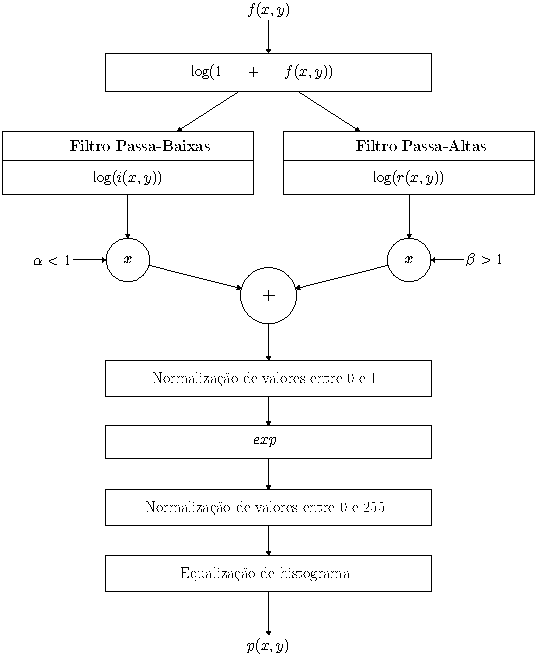
\includegraphics[width=12cm]{figs/fig_homomorphicFilter.pdf}
    \caption{Esquema de aplicação do filtro homomórfico. Fonte: \cite{gomes:2017}.}
    \label{fig:filtroH2}
\end{figure}

Nesta dissertação, o filtro homomórfico foi utilizado para corrigir a iluminação não uniforme, minimizando a influência da iluminação no processamento de imagens. A~\autoref{fig:filtroH} (b) apresenta o resultado obtido com a aplicação do filtro homomórfico a partir de uma imagem de entrada da base VOPTICAL\_LS (\autoref{fig:filtroH}).

\begin{figure}[ht!]
    \centering
    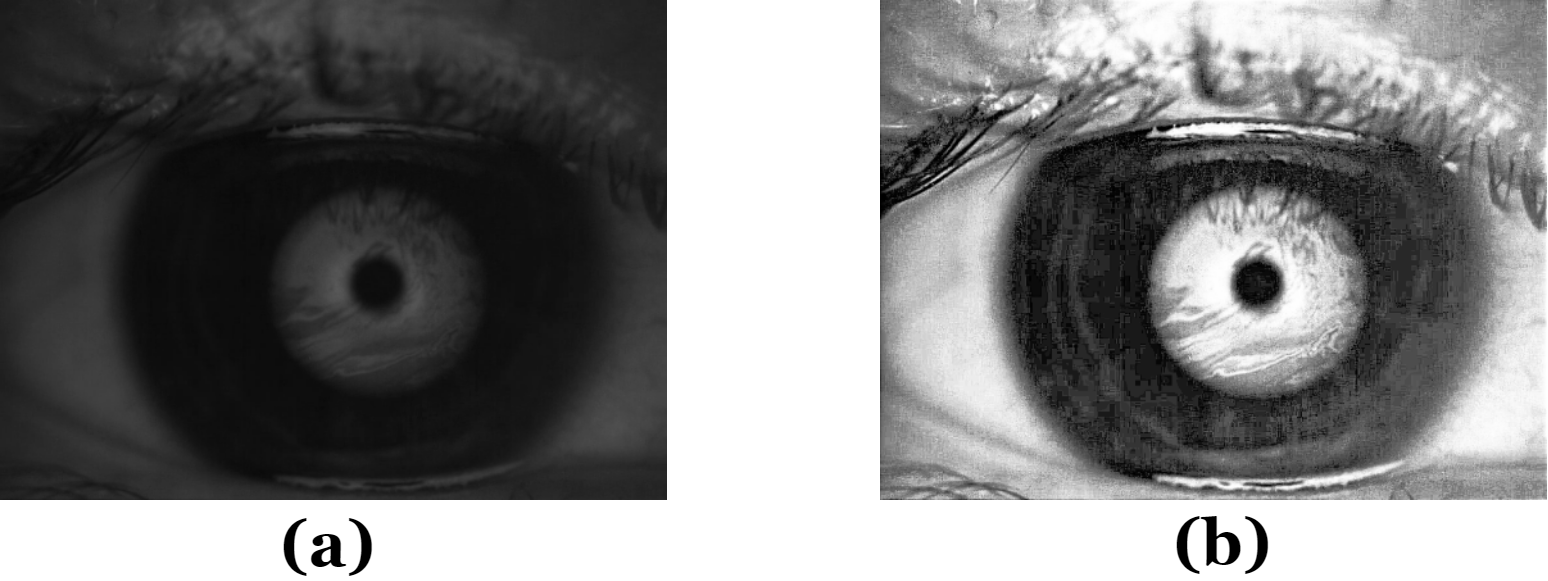
\includegraphics[width=11cm]{figs/FiltroH.png}
    \caption{Exemplo de utilização do filtro homomórfico (a) imagem original; (b) imagem após aplicação do filtro homomórfico.}
    \label{fig:filtroH}
\end{figure}
\end{comment}

\section{Extração de Características}
\label{sec:extCaracteristicas}

A extração de características tem o objetivo de extrair informações quantitativas de interesse ou que sejam básicas para discriminação entre as classes de objetos. Portanto, esta etapa visa obter medidas descritivas das bases de imagens, as quais formarão os vetores de características que serão usados nas etapas de seleção e classificação. A etapa de extração de características pode ser dividida em duas categorias de análise, sendo elas: textura e forma.

Em uma análise por textura, o objetivo é descrever aspectos da imagem no que diz respeito a suavidade, rugosidade e regularidade \cite{gonzalez2008digital}, possibilitando distinguir regiões da imagem que apresentam as mesmas características de padrões \cite{azevedo2003computaccao}. Já em uma análise baseada na forma, o intuito é extrair informações que mensuram sobre propriedades morfológicas da imagem, caracterizando a forma e aparência dos objetos
através do contorno ou da área do objeto em estudo \cite{BRAZ:2014}.

O procedimento de extração de características adotado nesta dissertação é distribuído em análise de texturas baseadas em geoestatística \cite{BRAZJUNIOR20091063} e outra em índices de diversidade \cite{16085910409503825}. Para tal, as seções seguintes apresentam as fundamentações dos descritores propostos para o tipo de análise por textura.

\section{Análise por Textura}

A análise de textura é, em princípio, uma técnica para avaliar a posição e a intensidade das características do sinal, ou seja, \textit{pixels} e sua intensidade em imagens digitais. As características de textura são, na verdade, parâmetros matemáticos calculados a partir da distribuição de \textit{pixels}, que caracterizam o tipo de textura e, portanto, a estrutura subjacente dos objetos mostrados na imagem \cite{CASTELLANO20041061}. De acordo com os métodos empregados para avaliar as inter-relações dos \textit{pixels}, três formas de análise de textura são usadas em processamento de imagem, categorizadas como: métodos estatísticos, estruturais e baseados em modelos \cite{gonzalez2010processamento}.

A abordagem estatística define a textura como um conjunto de medidas locais extraídas do padrão, descrevendo as imagens através de regras estatísticas que administram tanto a distribuição quanto a relação entre os diferentes níveis de cinza. A abordagem estrutural considera a textura como um conjunto de sub-padrões espaciais na imagem com arranjos espaciais repetitivos regulares, conforme regras bem definidas \cite{morais1999discriminaccao}. Finalmente, na abordagem baseada em modelos a textura pode ser considerada como uma realização de um processo estocástico dirigido por parâmetros, que são utilizados como características \cite{felipe2002utilizando}.

Nesta dissertação, foram utilizados para caracterizar a textura das imagens do filme lacrimal, a função K de \textit{Ripley} e os índices de diversidade filogenética, que são medidas estatísticas.

\subsection{Função K de \textit{Ripley}}
\label{sec:kripley}

A função K de \textit{Ripley} é comumente usada em análise de dados espaciais, sendo frequentemente empregada na ecologia, para descrever a distribuição espacial de árvores e outras espécies em uma floresta. Nos últimos trinta anos, sua aplicação também foi utilizada nas mais diversas áreas como: epidemiologia, geomorfologia, criminologia, geologia, etc \cite{lancaster2004spatial}.

Essa técnica pode ser usada para resumir um padrão de pontos, testar hipóteses sobre o padrão, estimar parâmetros e ajustar modelos~\cite{ripley1977modelling}. A função é definida na Equação~\ref{equacao:equacaoRipley}:

\begin{equation}
\label{equacao:equacaoRipley}
R(d,i) = \sqrt{\frac{Ak(i,j)}{N}}, i \neq j,
\end{equation}onde $d$ representa a função de distância usada na análise, $A$ indica a área da região em questão, calculada a partir do ponto de referência $i$ sob a distância $d$. $N$ o total de pontos da amostra, e $k$ é a função de pertinência que verifica se $j$ está contido no conjunto de análise determinado por $i$ e $d$. Ou seja, cada padrão espacial pontual é examinado separadamente dos demais, e tratado como a ocorrência ou não de uma mesma intensidade dentro da distância especificada.

Em suma, a função K de \textit{Ripley} calcula uma relação do total de indivíduos de uma determinada espécie distribuída em uma região de estudo. Segundo \cite{martins2007detecccao}, além do uso convencional (círculos) da função K de \textit{Ripley}, foi proposta também uma nova forma de aplicação da função, através da análise dos padrões de pontos em anéis. Basicamente, a modificação consiste em substituir a região de interesse dada pela \autoref{fig:ripleyCircAneis} (a) pela região compreendida entre dois círculos concêntricos, como na \autoref{fig:ripleyCircAneis} (b). Além dessas duas abordagens, formas complexas como, janelas e diagonais também podem ser aplicadas.

\begin{figure}[ht]
    \centering
    \caption{Abordagens da função K de \textit{Ripley}. (a) círculos; (b) anéis.}
     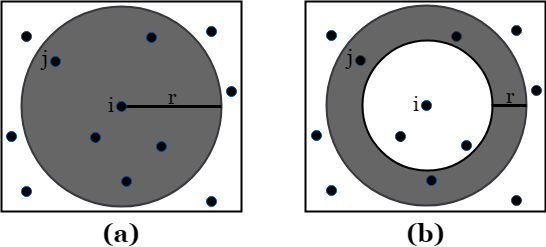
\includegraphics[width=8cm]{figs/RipleyCircAneis1.png}
     \legend{Fonte: Adaptado de \cite{martins2007detecccao}.}
    \label{fig:ripleyCircAneis}
\end{figure}

O cálculo do raio de cada círculo é baseado no raio máximo determinado pela região. Inicialmente, é necessário calcular a menor dimensão da Região de Interesse (ROI). Assim, o raio máximo é representado pela metade do valor da menor dimensão. A partir do raio máximo, calculam-se os demais através da alteração de proporção em relação ao primeiro, dada pela \autoref{equacao:equacaoCirc}.

%Para cada círculo, o cálculo dos raios é baseado no seu raio máximo. Inicialmente, é necessário calcular o menor tamanho da Região de Interesse (ROI). O raio máximo é metade do menor tamanho de ROI. Então, os outros raios podem ser calculados usando diferentes proporções do raio máximo (\autoref{equacao:equacaoCirc}).

\begin{equation}
\label{equacao:equacaoCirc}
Raio_{i} = \frac{Raio_{max}}{i},
\end{equation}
onde $i$ = $1,2,3...,n$, e $n$ é a quantidade de raios determinados pela aplicação.

Para calcular a divisão em anéis, segue-se o mesmo princípio do cálculo da divisão em círculos. A diferença está no fato de anéis não possuírem áreas comuns entre si, como tem os círculos concêntricos. Assim, o raio máximo do anel interno é utilizado como um raio mínimo para o próximo.

A partir do mesmo cálculo do raio máximo obtido pela divisão de círculos, os raios mínimos e máximos dos anéis são obtidos usando as Equações \ref{equacao:equacaoMin} e \ref{equacao:equacaoAnelMax}, respectivamente.

\begin{equation}
\label{equacao:equacaoMin}
Raio_{min} (i) = \frac{Raio_{max}}{n}i
\end{equation}
e
\begin{equation}
\label{equacao:equacaoAnelMax}
Raio_{max} (i) = \frac{Raio_{max}}{n}(i + 1),  
\end{equation}onde $i$ = $1,2,3...,n$, e $n$ é a quantidade de raios determinados pela aplicação.

Portanto, as divisões criam novas representações de regiões circulares e concêntricas da região, a partir das ROIs das imagens. Assim, cada divisão gera recortes individualizados que passarão por todo o processo de extração de características.

\subsection{Índices de Diversidade e Diversidade Filogenética}
\label{sec:indicesDiversidade}

A diversidade é um termo comumente empregado na Ecologia para medir a biodiversidade de um ecossistema, com intuito de identificar a distribuição de um grupo de espécies e as suas relações. De modo geral, o objetivo de um índice de diversidade é descrever a variedade de espécies presentes em uma comunidade ou determinada região, que tais representam um conjunto de espécies que ocorrem em um determinado lugar e tempo \cite{magurran2013measuring}.

O uso dos índices de diversidade são comuns na literatura para extrair características em nódulos pulmonares \cite{de2017computer,de2017lung,de2018classification} e na diferenciação de massas benignas e malignas em mamografias \cite{CARVALHO2018210, de2015classification}. Diferentemente dessas aplicações, os índices de diversidade filogenética foram utilizados no método proposto para extrair características em imagens do filme lacrimal para classificar as categorias da camada lipídica. Para tanto, foram utilizados três grupos dos índices: (1) baseados na distância entre pares de espécies; (2) baseados na topologia; e (3) baseados em caminho mínimo.

\begin{comment}
%Os índices do primeiro grupo são capazes de mensurar a cerca das relações de parentesco que determinadas espécies possuem, como por exemplo, a quantidade de ancestrais comuns que existem entre determinadas espécies. O segundo grupo, explora o grau de parentesco entre as espécies relacionando possíveis ancestrais em comum. Já o terceiro, possuem a propriedade de aferir o quão distante estão as espécies presentes na comunidade, considerando a distância filogenética, calculada a partir de uma árvore filogenética, podendo ser representada em forma de dendrograma, como apresentada na Figura~\ref{fig:Cladograma}.

%foi um dos primeiros a propor o uso de métodos baseados em topologia, refletindo a ordem de ramificação filogenética dentro de um grupo. Nesta abordagem, cada tipo de comunidade é ponderada pelo número de nós entre as espécies e a raiz da árvore filogenética (dendrograma); Desta forma, as espécies com os maiores pesos são aquelas com maior distância da raiz. Em nosso trabalho, as distâncias são representadas pelo número de nós entre as espécies.

%determinam além das propriedades filogenéticas a topologia pela qual as espécies se distribuem no dendrograma

%denotam relações evolutivas.

%Nesta árvore, os nós das folhas representam as espécies analisadas, os nós internos correspondem a algum antepassado comum e as arestas indicam a distância filogenética entre duas espécies. Assim, é possível fazer uma conexão evolutiva entre as espécies \cite{carvalho2016metodos}.

%Para implementar essa ideia, a primeira etapa é realizar uma correspondência entre os termos usados na biologia e os utilizados neste trabalho. A Tabela~\ref{table:descricao} apresenta essa correspondência.

%os ancestrais são representados pelos nós internos no cladograma
%A escolha dos índices de diversidade filogenética foi devido ao seu grande potencial na caracterização de texturas em imagens.
\end{comment}

Os índices do primeiro grupo são capazes de mensurar acerca das relações de parentesco que determinadas espécies possuem, como por exemplo, a quantidade de ancestrais comuns que existem entre determinadas espécies. O segundo grupo, reflete a ordem de ramificação filogenética dentro de um grupo. Já o terceiro, possui a propriedade de aferir o quão distante estão as espécies presentes na comunidade, considerando a distância filogenética, calculada a partir de uma árvore filogenética \cite{carvalho2016metodos}.

%que é uma representação gráfica usada para descrever a relação filogenética entre espécies ancestrais

%Árvores filogenéticas são usadas na biologia para descrever as relações evolutivas entre as espécies, a fim de determinar possíveis ancestrais comuns. As árvores filogenéticas podem ser representadas em forma de cladograma inclinado para descrever a relação filogenética entre espécies ancestrais \cite{baxevanis2004bioinformatics}. A Figura~\ref{fig:Cladograma} ilustra uma árvore filogenética dos macacos em forma de cladograma. Note que um chimpanzé tem maior proximidade filogenética com humanos do que um siamango. Nesta árvore, os nós da folha são as espécies analisadas, os nós internos correspondem a algum ancestral comum, e as arestas indicam a distância filogenética entre duas espécies \cite{carvalho2016metodos, baxevanis2004bioinformatics}.

Árvores filogenéticas e filogenia são usadas na biologia para descrever as relações evolutivas entre as espécies, a fim de determinar possíveis ancestrais comuns \cite{baxevanis2004bioinformatics}. A Figura~\ref{fig:Cladograma} ilustra uma árvore filogenética dos macacos em forma de cladograma inclinado. Note que um chimpanzé tem maior proximidade filogenética com humanos do que um siamango. Nesta árvore, os nós da folha são as espécies analisadas, os nós internos correspondem a algum ancestral comum, e as arestas indicam a distância filogenética entre duas espécies \cite{carvalho2016metodos, baxevanis2004bioinformatics}.

%Árvores filogenéticas são usadas na biologia para descrever as relações evolutivas entre as espécies, a fim de determinar possíveis ancestrais comuns. As árvores filogenéticas podem ser representadas em forma de cladograma inclinado \cite{baxevanis2004bioinformatics} como apresentado na Figura~\ref{fig:Cladograma}, que ilustra uma árvore filogenética dos macacos. Note que um chimpanzé tem maior proximidade filogenética com humanos do que um siamango. Nesta árvore, os nós da folha são as espécies analisadas, os nós internos correspondem a algum ancestral comum, e as arestas indicam a distância filogenética entre duas espécies \cite{carvalho2016metodos, baxevanis2004bioinformatics}.

\begin{figure}[ht!]
    \centering
    \caption{Árvore filogenética representada como cladograma.}
     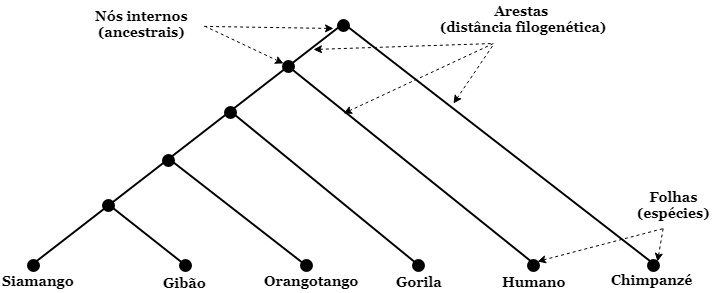
\includegraphics[width=12cm]{figs/Cladograma2.png}
     \legend{Fonte: Adaptado de \cite{baxevanis2004bioinformatics}.}
    \label{fig:Cladograma}
\end{figure}
%\FloatBarrier

Árvores filogenéticas combinadas com índices de diversidade filogenética comparam padrões de comportamento entre espécies de diferentes áreas e, descrevem suas relações evolutivas entre seus antepassados \cite{vane1991protect}. Para implementar essa ideia, o primeiro passo é fazer uma correspondência entre os termos usados na biologia e os utilizados neste trabalho (Tabela~\ref{table:descricao}).

A~\autoref{table:descricao} apresenta a correspondência dentro do contexto de processamento de imagens. A comunidade é representada pela ROI, seus indivíduos são representados pelos \textit{pixels}, os níveis de cinza são suas espécies e a distância filogenética é representada pelo número de arestas entre duas espécies.

\definecolor{lightgray}{gray}{0.94}
\begin{table}[!ht]
\centering
\onehalfspacing
\rowcolors{1}{}{lightgray}
\caption{Correspondência entre os termos da biologia e o método proposto.}
\label{table:descricao}
\begin{tabular}{lp{7cm}l}
\hline
\multicolumn{1}{c}{\textbf{Biologia}} & \multicolumn{1}{c}{\textbf{Método Proposto}}          \\ \hline \hline
Comunidade                            & Região de interesse da imagem do filme lacrimal      \\
Espécies                              & Número máximo de valores de níveis de cinza na região \\
Indivíduos                             & Quantidade de \textit{pixels} de uma determinada espécie \\
%Ancestrais                            & Número de nós internos no dendrograma                 \\
Distância filogenética                & Número de arestas entre duas espécies                 \\ \hline
\end{tabular}
\end{table}
\FloatBarrier

A Figura~\ref{fig:ExemploCladograma} mostra um exemplo da construção de um árvore filogenética em forma de cladograma a partir de uma amostra de imagem original. Esta imagem contém três níveis de cinza, que são preto (P), cinza (C) e branco (B), bem como as espécies que compõem a comunidade. O número de \textit{pixels} para P é 4, C é 2 e B é 3, compreendendo assim os indivíduos da comunidade. A representação genérica da árvore e sua matriz de distância para a imagem da Figura~\ref{fig:ExemploCladograma} (a) são mostradas na Figura~\ref{fig:ExemploCladograma} (b) e (c), respectivamente.

\begin{figure}[ht!]
    \centering
    \caption{Imagem sintética para exemplificar o cladograma. (a) amostra de uma imagem original; (b) árvore enraizada na forma de cladograma inclinado e (c) matriz de distâncias.}
     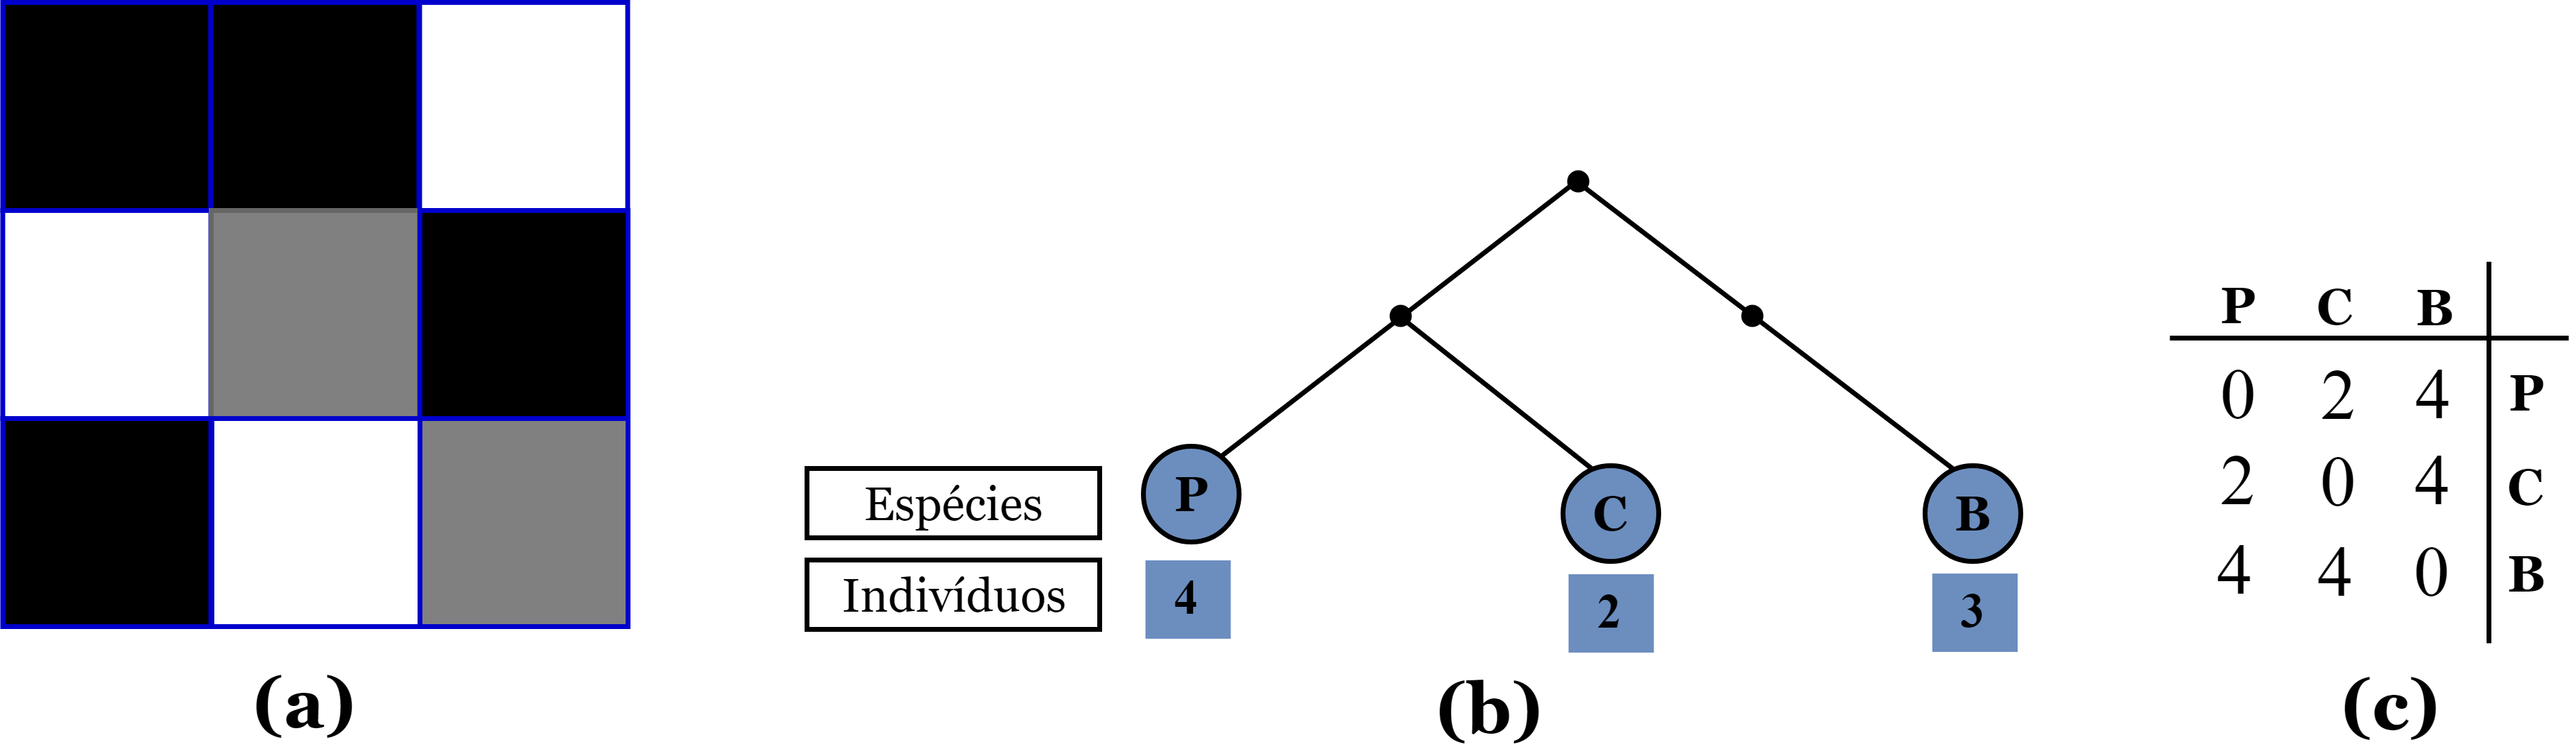
\includegraphics[width=16cm]{figs/ExemploCladogramaFinal.png}
     \legend{Fonte: Adaptado de \cite{CARVALHO2018210}.}
    \label{fig:ExemploCladograma}
\end{figure}
\FloatBarrier

A informação requerida de um determinado cladograma para o cálculo da diversidade filogenética pode ser resumida por uma matriz de distâncias entre espécies, obtida a partir do cladograma. Os valores dentro da matriz de distância são interpretados como a distinção entre cada par de espécies ou entre uma espécie específica e todas as outras \cite{CARVALHO2018210}. Assim, os detalhes fundamentais de cada grupo de índices são coletados para composição dos descritores propostos. Nas próximas seções serão apresentados maiores detalhes de cada grupo, e como é realizado o cálculo de cada um dos índices.

%já que estes índices se complementam, isto é, um grupo é capaz de mensurar alguma riqueza de propriedade que outro grupo não consegue.

\subsubsection{Índices de Diversidade Filogenética Baseados na Distância entre Pares de Espécies}
\label{sec:indicesPE}

Os índices que medem as relações de distância entre pares de espécies são baseados na matriz de distância de todas as espécies da comunidade. Estes índices podem ser interpretados como a distinção entre cada par de espécies ou de cada espécie em particular para todas as outras. Nessa abordagem, as distâncias são representadas pelo número de arestas entre as espécies, calculadas sobre a árvore mapeada (\autoref{fig:Cladograma}). Nesse grupo, cinco índices são utilizados: a entropia quadrática intensiva \cite{izsak2000link}, a entropia quadrática extensiva \cite{izsak2000link}, a distinção taxonômica média \cite{pienkowski1998taxonomic}, a distinção taxonômica total \cite{krwarwick} e a medida de diversidade pura \cite{gerlinger2012intratumor}.

A entropia quadrática intensiva ($I$) estabelece uma ligação entre os índices de biodiversidade e índices de diversidade \cite{izsak2000link}. O índice $I$ representa o número de espécies e as relações taxonômicas, quando existem os mesmos valores formais ou hipotéticos em abundância. Portanto, $I$ expressa a distância taxonômica média entre duas espécies. As relações entre espécies influenciam o valor de $I$, diferentemente de outros índices de diversidade \cite{izsak2000link}. O índice $I$ é dado pela~\autoref{equacao:equacaoI}.
\begin{equation}
\label{equacao:equacaoI}
I = \left [ \sum d_{i,j} \right ] / s^{2},
%I = [\frac{\sum\limits_{i=1}^{i=n-1}\sum\limits_{j=1}^{j=n-1} d_{i,j}}{s^{2}}]
\end{equation}
onde a distância entre as espécies $i$ e $j$ é representada por $d_{i,j}$ e $s$ o número de espécies.

Em relação às propriedades do índice, a monotonicidade é geralmente necessária para métricas de diversidade. Para uma determinada medida $J$, essa propriedade significa que: $J (A \cup \left \{ x \right \}) > J(A)$, garante que o valor do índice aumentará adicionando uma nova espécie $x$ a um conjunto de espécies $A$. Portanto, $I$ não é um índice de diversidade ideal, uma vez que não satisfaz esse requisito. Para resolver este problema, a entropia quadrática extensiva ($E$) \cite{izsak2000link} foi proposta com base em $I$. $E$ representa a soma das diferenças de espécies. O índice $E$ tem a propriedade de monotonicidade, já que para qualquer conjunto de espécies $A$, se uma nova espécie $x$ for adicionada, o valor de $E$ será modificado. O índice $E$ é calculado na Equação~\ref{equacao:equacaoE}.
\begin{equation}
\label{equacao:equacaoE}
E = \sum d_{i,j},
%E = \sum\limits_{i=1}^{i=n-1}\sum\limits_{j=1}^{j=n-1} d_{i,j}
\end{equation}
onde a distância entre as espécies $i$ e $j$ é representada por $d_{i,j}$.

A distinção taxonômica média ($DTM$) e a distinção taxonômica total ($DTT$) foram originalmente desenvolvidas com base nas relações taxonômicas. No entanto, podem ser facilmente adaptadas às informações filogenéticas \cite{schweiger2008comparative}. A $DTM$ refere-se à distância taxonômica média entre duas espécies \cite{pienkowski1998taxonomic} e $DTT$ representa a distinção taxonômica média de todas as espécies dentro da comunidade. $DTM$ e $DTT$ são, respectivamente, definidos nas Equações~\ref{equacao:equacaoIDTM} e \ref{equacao:equacaoIDTT}.
\begin{equation}
\label{equacao:equacaoIDTM}
DTM = \left [ \sum \sum_{i<j}d_{i,j} \right ] / \left [ s(s - 1)/2 \right ]
%DTM = [\frac{\sum\limits_{i=1}^{i=n-1}\sum\limits_{j=1}^{j=n-1}d_{i,j}}{\frac{s(s-1)}{2}}]
\end{equation}
e
\begin{equation}
\label{equacao:equacaoIDTT}
DTT = \sum_{i}\left [ \left ( \sum_{i \neq j}d_{i,j} \right )\left (s - 1  \right ) \right ],
%DTT = [\frac{\sum\limits_{i=1}^{i=n-1}\sum\limits_{j=1}^{j=n-1}d_{i,j}}{(s-1)}]
\end{equation}
onde $d_{i,j}$ representa a distância entre as espécies $i$ e $j$, e o número de espécies é definido por $s$.

Finalmente, o índice de diversidade pura ($IDP$) verifica a distância de uma espécie para seu vizinho mais próximo \cite{faith1992conservation}. $IDP$ é definido na Equação~\ref{equacao:equacaoIDP}.
\begin{equation}
\label{equacao:equacaoIDP}
IDP = \sum d_{i} _{ } _{ }_{min},
%IDP =\sum\limits_{i=1}^{i=n-1}\textit{$d_{i}$} \textit{$_{min}$}
\end{equation}
onde $d_{i} _{ } _{ }_{min}$ representa a menor distância do vizinho mais próximo da espécie $i$ em relação as todas as outras espécies.

\subsubsection{Índices de Diversidade Filogenética Baseados na Topologia}
\label{sec:indicesT}

Os índices de diversidade filogenética baseados na topologia refletem a ordem de ramificação filogenética dentro de um grupo. Nesta abordagem, cada espécie de uma comunidade é ponderada de acordo com o número de nós entre as espécies e a raiz da árvore filogenética. Portanto, espécies com pesos maiores são aquelas com maiores distâncias da raiz no cladograma \cite{vane1991protect}. Esse grupo é composto por dois índices: a soma básica dos pesos e soma dos pesos normalizados \cite{keith2005taxonomic,posadas2001using,vane1991protect}, que estão relacionados às espécies da comunidade que indicam o grau de similaridade entre elas.

A soma básica de pesos ($Q$) é o quociente de todos os nós dividido pelo número de nós entre a raiz e uma espécie, que representa a soma das contribuições de cada espécie para a diversidade. O índice $Q$ é definido na Equação~\ref{equacao:equacaoQ1}.
\begin{eqnarray}
\label{equacao:equacaoQ1}
Q = \sum Q_{i} \nonumber \\
Q_{i} = I/I_{i} \\
I = \sum I_{i}, \nonumber, 
\end{eqnarray}
onde $ Q_{i}$ é o quociente do total de nós raiz para todas as espécies por $ I_{i}$, que é o número de nós entre a raiz e a espécie $i$.

A soma dos pesos normalizados ($W$) representa para cada espécie o peso normalizado, isto é, os valores de $Q$ de cada espécie dividido pelo valor de $Q_{min}$. $W$ é calculado pela Equação~\ref{equacao:equacaoW2}.
\begin{eqnarray}
\label{equacao:equacaoW2}
W = \sum W_{i} \nonumber \\
W_{i} = Q_{i}/Q_{min},
\end{eqnarray}
onde $Q_{min}$ representa o quociente do caminho mínimo da raiz para a espécie.

%índices de diversidade filogenética baseados em topologia, que determinam além das propriedades filogenéticas a topologia pela qual as espécies se distribuem no dendrograma. Em outras palavras, através desses índices, é possível explorar o grau de parentesco entre as espécies relacionando possíveis ancestrais em comum. Portanto, viabilizando a caracterização da relação homogeneidade e heterogeneidade com base na topologia das espécies. %%% ja estava comentado

\subsubsection{Índices de Diversidade Filogenética Baseados em Caminho Mínimo}
\label{sec:IndicesCM}

Os índices de diversidade filogenética baseados em caminhos mínimos analisam a distância das espécies em uma comunidade. Em resumo, quanto menor o caminho, menor o número de espécies e, como resultado, menor a diversidade. Três índices são usados: medida quantitativa da diversidade filogenética \cite{faith1992conservation}, diversidade filogenética incluindo ramos de base \cite{rodrigues2002maximising} e diversidade filogenética média \cite{rodrigues2002maximising}.

A medida quantitativa da diversidade filogenética ($PD_{NODE}$) representa a extensão total mínima de todos os ramos filogenéticos, o que é fundamental para medir um táxon\footnote{Um grupo ou divisão usado em biologia para classificação científica de espécies.} em uma árvore filogenética. Valores maiores de $ PD_{NODE}$ representam maiores diversidades \cite{faith1992conservation}. $PD_{NODE}$ é definido na Equação~\ref{equacao:equacaoPDNODE}.
\begin{equation}
\label{equacao:equacaoPDNODE}
 PD_{NODE} = \sum n_{i},
\end{equation}
onde $n_{i}$ indica o número de nós $i$ no caminho mínimo de cada espécie existente na diversidade.

Os Índices de diversidade filogenética incluindo ramos de base ($PD_{ROOT}$), correspondem ao número de nós dentro do caminho raiz máximo \cite{rodrigues2002maximising}. O $PD_{ROOT}$ é definido na Equação~\ref{equacao:equacaoPDROOT}.
\begin{equation}
\label{equacao:equacaoPDROOT}
PD_{ROOT} = \sum n_{iROOT},
\end{equation}
onde $n_{iROOT}$ é o número de nós dentro no caminho.

Finalmente, tem-se a diversidade filogenética média ($AvPD$), definida na Equação~\ref{equacao:equacaoAvPD}.
\begin{equation}
\label{equacao:equacaoAvPD}
AvPD = PD_{NODE/s},
\end{equation}
onde $s$ indica o número de espécies na comunidade.

\section{Representação da Imagem}
\label{sec:representacao da imagem}

Esta seção apresentada as técnicas para representação das imagens utilizadas no método proposto, visando aprimorar o desempenho da extração de características da função K de \textit{Ripley} e o reconhecimento de padrões. Para o desenvolvimento da representação da imagem foram utilizadas técnicas de quantização para a digitalização dos valores de amplitude e o \textit{Local Binary Pattern} para encontrar a distribuição espacial de padrões locais de textura existente na região de interesse. 

\subsection{Quantização}
\label{sec:quantizacao}

O processo de quantização constitui em obter a representação de uma imagem com $L$ níveis para cada \textit{pixel} com $L$ = $2^{b}$, sendo $b$ o número de \textit{bits} usados para o armazenamento do valor do \textit{pixel}. Dessa forma, se houver a necessidade de quantizar para $L'$ níveis de cinza, utiliza-se a quantização uniforme, que consiste em dividir a escala de cinza da imagem em intervalos iguais, onde cada intervalo é mapeado para um valor de cinza na imagem quantizada \cite{gonzalez2010processamento}. O mapeamento é definido na Equação~\ref{equacao:quantizacao}.

\begin{equation}
\label{equacao:quantizacao}
q(i,j) = (2^{b} - 1) \frac{p(i,j) - I_{min}}{I_{max} - I_{min}}, 
\end{equation}
sendo $q(i,j)$ o nível de cinza do \textit{pixel} $(i,j)$ da nova imagem quantizada, $p(i,j)$ o nível de cinza do \textit{pixel} da imagem original, $[{I_{max} - I_{min}}]$ os limites inferiores e superiores da escala de cinza da imagem original e $b$ o número de \textit{bits} utilizados para armazenar cada \textit{pixel} da imagem quantizada.

\subsection{\textit{Local Binary Pattern}}

\citeonline{ojala1996comparative} foi proposto originalmente o \textit{Local Binary Pattern} (LBP) como um operador não paramétrico para descrever a estrutura espacial local da imagem, demonstrando alta capacidade de discriminar características de textura. A ideia básica do LBP é que a imagem é composta por micropadrões, que são as unidades de textura. O LBP é definido na Equação~\ref{equacao:lbp}.

\begin{equation}
\label{equacao:lbp}
LBP(x_{c},y_{c}) = \sum_{n=0}^{n-1}S(i_{n}-i_{c})2^{n},
\end{equation}
onde $n$ representa o número de vizinhos do \textit{pixel} central $(x_{c},y_{c})$ considerados no cálculo, $i_{c}$ é o valor de nível de cinza do \textit{pixel} central $(x_{c},y_{c})$, $i_{n}$ é o valor de nível de cinza de cada \textit{pixel} vizinho e $S(x)$ é uma função que devolve 1 se $x$ $\geq$ 0 e 0, caso contrário.

\begin{figure}[ht!]
    \centering
    \caption{Cálculo do LBP. (a) imagem; (b) imagem binária; (c) matriz de pesos; (d) valores resultantes.}
    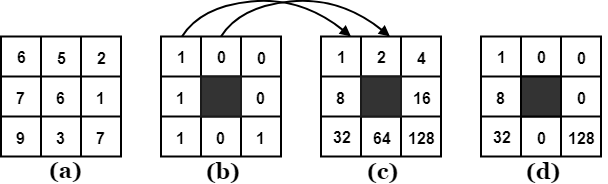
\includegraphics[width=12cm]{figs/LBP2.png}
    \legend{Fonte: Adaptado de \cite{ojala1996comparative}.}
    \label{fig:lbp}
\end{figure}

A~\autoref{fig:lbp} apresenta um exemplo do cálculo LBP. A partir de uma janela de tamanho 3 x 3 (\autoref{fig:lbp} (a)), é realizado a subtração dos valores de níveis de cinza dos \textit{pixels} vizinhos (individualmente) com o valor do nível de cinza do \textit{pixel} central, formando uma matriz binária composta pelos valores 0 ou 1, dependendo do resultado da diferença dos \textit{pixels} analisados (\autoref{fig:lbp} (b)). Em seguida, os valores da matriz binária são multiplicados pelo respectivo valor da matriz de pesos (\autoref{fig:lbp} (c)). Finalmente, o resultado do LBP se dá através da soma de todos os valores resultantes da multiplicação (\autoref{fig:lbp} (d)), no exemplo em questão, o LBP é 169.

\section{Seleção de Características}
\label{sec:selecao}

Em aplicações de visão computacional é bastante recorrente a utilização de técnicas que geram um grande número de características, que muitas vezes são desnecessárias para realizar a separação dos indivíduos em suas classes. Portanto, a escolha do conjunto de características relevantes é importante para simplificar o modelo e aumentar seu poder de generalização. Neste contexto, realiza-se a seleção das características que é uma etapa opcional no processo de reconhecimento de padrões.%, a fim de aumentar a eficiência dos classificadores e diminuir custos computacionais.

A seleção de características visa reduzir a dimensionalidade do espaço de características sem perca de informações. As principais razões para tal redução são os custos de medição e precisão do classificador. Por este motivo, faz-se necessário a utilização de algoritmos de seleção de características que propiciem a obtenção de representações dos padrões de forma robusta. Sendo assim, o algoritmo \textit{Greedy Stepwise} \cite{ambelu2010comparison} foi o escolhido para efetuar este procedimento, afim de aumentar a eficiência dos classificadores e diminuir custos computacionais.

\subsection{Algoritmo \textit{Greedy Stepwise}}
\label{sec:greedyStepwise}

O \textit{Greedy Stepwise} é um algoritmo guloso de paradigma algorítmico que segue a heurística de resolução de problemas de fazer a escolha localmente ótima em cada estágio \cite{gutin2002traveling}, com a intenção de encontrar um ótimo global. Em muitos problemas, uma estratégia gulosa geralmente não produz uma solução ótima. Mesmo assim, uma heurística gananciosa pode produzir soluções ótimas localmente que se aproximam de uma solução globalmente ótima em um período de tempo razoável.

Esse algoritmo executa uma busca gulosa, no sentido \textit{forward} ou \textit{backward}, através do espaço de busca dos subconjuntos de atributos. A busca pode iniciar com nenhum/todos os atributos ou de um ponto arbitrário no espaço, e encerra quando todas as inclusões ou exclusões de atributos resultarem em uma diminuição da taxa de acerto. Para tanto, neste trabalho, esta abordagem encontra características que discriminam melhor as categorias da camada lipídica do filme lacrimal para o conjunto de características geradas, que contém menos redundâncias que poderiam prejudicar os classificadores durante as próximas etapas \cite{ambelu2010comparison}.

\section{Reconhecimento de Padrões}
\label{sec:recPadroes}

O reconhecimento de padrões é o campo da ciência que tem como objetivo a classificação e reconhecimento de objetos em um determinado número de categorias ou classes a partir da observação de suas características \cite{Theodoridis:2008:PRF:1457541}. Dessa forma, visa construir uma representação mais simples de um conjunto de dados através de suas características mais relevantes, possibilitando sua partição em classes \cite{Duda:2000:PC:954544}.

O reconhecimento de padrões tem uma ampla aplicação em astronomia, medicina, robótica, reconhecimento de fala, sensoriamento remoto por satélites, etc. O processo de reconhecimento de padrões é composto por duas etapas: classificação e reconhecimento. Durante a etapa de classificação uma amostra de uma população é particionada em grupos chamados classes. Na etapa de reconhecimento uma amostra desconhecida, porém pertencente à mesma população, é reconhecida como integrante de uma das classes criadas anteriormente \cite{looney1997pattern}.

As técnicas de classificação são compostas por dois grupos: supervisionada e não-supervisionada. A classificação supervisionada consiste em um processo prévio de treinamento de um classificador para o conhecimento dos padrões desejados. Posteriormente, o classificador é capaz de identificar a classe de qualquer objeto desconhecido da mesma população de treinamento. Já na classificação não supervisionada não há informação prévia sobre as classes às quais os padrões de amostras pertencem \cite{pedrini2008analise}.

Neste trabalho foram utilizadas as técnicas de classificação supervisionada \textit{Support Vector Machine}, \textit{Random Forest}, \textit{Naive Bayes} e \textit{Bayes Net} para o reconhecimentos dos padrões de interferência da camada lipídica do filme lacrimal.

\subsection{Classificadores}
\label{sec:classificadores}

O método proposto utiliza \textit{Support Vector Machine} (SVM), \textit{Random Forest} (RF), \textit{Bayes Net} (BN) \cite{nielsen2009bayesian} e \textit{Naive Bayes} (NB) \cite{john2010elements} para o reconhecimento de padrões, objetivando categorizar os padrões de interferência da camada lipídica do filme lacrimal.

%Multilayer Perceptron (MLP) \cite{monika2015di}, Random Tree (RT) \cite{biau2012analysis} e RBFNetwork (RBFNet) \cite{broomhead1988radial}.

A BN pertence à família dos modelos gráficos probabilísticos, que representa um conjunto de variáveis e suas dependências condicionais. Essas estruturas gráficas são usadas para representar o conhecimento sobre um domínio incerto. Particularmente, cada nó no gráfico representa uma variável aleatória, enquanto as arestas entre os nós representam dependências probabilísticas entre as variáveis aleatórias correspondentes. Estas dependências condicionais no gráfico são frequentemente estimadas usando métodos estatísticos e computacionais conhecidos. Assim, as BNs combinam princípios da teoria dos grafos, teoria da probabilidade, ciência da computação e estatística \cite{nielsen2009bayesian}.

%As redes bayesianas são um tipo de modelo gráfico probabilístico que utiliza a inferência bayesiana para cálculos de probabilidade. As redes bayesianas visam modelar a dependência condicional e, portanto, a causalidade, representando a dependência condicional por arestas em um grafo direcionado. Através dessas relações, pode-se conduzir eficientemente a inferência sobre as variáveis aleatórias no gráfico através do uso de fatores.

A NB é um técnica de classificação probabilística baseada no teorema de Bayes com uma suposição de independência entre os preditores, ou seja, as características de cada classe são assumidas como condicionalmente independentes. Por ser muito simples e rápido, possui um desempenho relativamente maior do que outros classificadores. Além disso, o NB precisa apenas de um pequeno número de dados de teste para concluir classificações com uma boa precisão \cite{jensen1996introduction}.

%Naive Bayes é uma técnica simples para a construção de classificadores: modelos que atribuem rótulos de classes a instâncias de problemas, representados como vetores de valores de recursos, em que os rótulos de classes são extraídos de um conjunto finito. 
    
%O RT é baseado na construção de múltiplas árvores de decisão, selecionando subconjuntos aleatórios de variáveis para cada árvore e usando a saída da árvore mais frequente como a classificação geral, ou seja, são geradas uma coleção de árvores de decisão onde cada árvore é formada a partir de diferentes amostras e subconjuntos dos dados de treinamento. A classificação funciona da seguinte maneira: o classificador de árvores aleatórias pega o vetor de recurso de entrada, classifica-o em cada árvore da floresta e exibe o rótulo de classe que recebeu a maioria dos "votos". No caso de uma regressão, a resposta do classificador é a média das respostas sobre todas as árvores na floresta \cite{biau2012analysis}.

O RF é uma técnica baseada na construção de um conjunto de árvores que são classificadores fracos e posteriormente são usados para construir um classificador estável e forte, melhor que a árvore média criada. O RF é um algoritmo flexível que mesmo sem ajuste de hiperparâmetros apresenta um ótimo resultado na maioria das vezes. Além disso, é possível utilizá-lo tanto para tarefas de classificação como de regressão \cite{breiman2001random}. 
    
O SVM é uma técnica baseada na teoria do aprendizado estatístico, usado para encontrar hiperplanos ideais para as classes linearmente separáveis e não separáveis. No segundo caso, são mapeados os dados de entrada para um espaço dimensional superior (usando função do \textit{kernel}) e definido um hiperplano de separação \cite{vapnik1998statistical}. O SVM utiliza o princípio de minimização do risco estrutural, que se baseia no fato de que a taxa de erro de uma máquina de aprendizado nos dados de teste é limitada pela soma da taxa de erro de treinamento e por um termo que depende da dimensão Vapnik-Chervonenkis (dimensão VC) \cite{zhuang2006parameter}.
    
%A MLP é uma abordagem de rede neural que consiste em um sistema de neurônios interconectados simples, ou nós, que mapeiam um conjunto de dados de entrada para um conjunto de saídas apropriadas. A MLP é semelhante à perceptron, mas com mais de uma camada de neurônios em alimentação direta. Tal tipo de rede é composta por camadas de neurônios ligadas entre si por sinapses com pesos. O aprendizado nesse tipo de rede é geralmente feito através do algoritmo de retropropagação do erro \cite{monika2015di}.
    
%A RBFNet permite a escolha do número de clusters (algoritmo de clusterização k-means) e, em seguida, implementa uma função de base radial (atribuição de valores partindo do distanciamento de um centro) para efetuar a classificação. As RBFNets normalmente possuem três camadas: uma camada de entrada, uma camada oculta com uma função de ativação RBF não linear e uma camada de saída linear. A entrada pode ser modelada como um vetor de números reais e a saída da rede é então uma função escalar do vetor de entrada \cite{broomhead1988radial}.

\section{Métricas de Desempenho} 
\label{sec:validacao}

O resultado da etapa de classificação é a identificação das categorias da camada lipídica do filme lacrimal. Após o processo de reconhecimento de padrões existe a necessidade de validar os resultados produzidos, através das métricas de desempenho. Esta atividade tem por finalidade avaliar o desempenho do método desenvolvido por meio de uma análise estatística dos resultados.

Para avaliar o desempenho do método proposto foram utilizadas estatísticas tipicamente aplicadas em sistemas CADx para análise de imagens médicas: acurácia \cite{duda1973pattern}, que é definida como a razão entre o número de casos corretamente classificados pelo número total de casos, e o desvio padrão relacionado a acurácia \cite{viera2005understanding}. Além disso, como existe desequilíbrio entre as classes das categorias, a medida \textit{F-Measure} foi usada, que representa a média harmônica de Precisão e \textit{Recall} \cite{fawcett2006introduction}.

%Além disso, como as classes são desbalanceadas, também usamos F-Measure, que representa a média harmônica de Accuracy e Recall

Outra medida utilizada é o índice \textit{Kappa}, que é um coeficiente de concordância utilizado em escalas nominais. O índice \textit{Kappa} mede a relação entre concordância e causalidade, e também o desacordo esperado, indicando quão legítimas são as interpretações \cite{rosenfield1986coefficient}. Esse índice é recomendado como uma medida que representa integralmente uma matriz de confusão. A categorização dos níveis de acurácia de classificação, pelo índice \textit{Kappa}, pode ser visualizada na~\autoref{tab:indkappa}, conforme definido por \citeonline{landis1977measurement}.

\begin{table}[ht!]
\centering
\rowcolors{1}{}{lightgray}
\onehalfspacing
\caption{Níveis de precisão de classificação, segundo o índice \textit{Kappa}.}
\label{tab:indkappa}
%\resizebox{7.5cm}{!}
\end{table}

O desempenho do método proposto também é avaliado usando a curva ROC (\textit{Receiver Operating Characteristic}), que indica a taxa positiva verdadeira (sensibilidade) como uma função da taxa de falsos positivos (1 - especificidade) \cite{fawcett2006introduction}. A curva é construída variando o limiar do classificador e avaliando os resultados gerados. A principal informação extraída de uma curva ROC é a área sob a curva ROC (\textit{Area Under the ROC Curve} - AUC), quanto maior a área, ou seja, mais próximo de 1 (equivalente a 100\%), melhor é o desempenho do classificador.


\section{Considerações Finais}

Neste capítulo foram apresentadas os fundamentos teóricos que são necessários para compreensão das técnicas utilizadas e suas aplicações no método proposto. Foram abordados temas como: Síndrome do Olho Seco, tipos de imagens do exame, técnicas de pré-processamento digital de imagens, descritores para análise de textura, técnicas para reconhecimento de padrões e métricas de desempenhos.
